\chapter{Brain as a complex system}\label{cha:brain-as-complex}
\section{Complex systems}\label{sec:complex-systems}
Behavior, or better stated \emph{collective} behavior, of wide range of system spanning the scales of movement of atoms to behavior of humans/animals can be studied under an inclusive young framework of sdudying \emph{complex systems}
\cite{bar-yamDynamicsComplexSystems2003,mitchellComplexityGuidedTour2011,hollandComplexityVeryShort2014,bar-yamWhyComplexityDifferent2017}.
\citet[Chapter 1]{mitchellComplexityGuidedTour2011} introduces and defines a complex system as following:
\begin{displayquote}\textsl{
    ``Systems in which organized behavior arises without an internal or external controller
    or leader are sometimes called self-organizing.
    Since simple rules produce complex behavior in hard-to-predict ways,
    the macroscopic behavior of such systems is sometimes called emergent.
    Here is an alternative definition of a complex system:
    a system that exhibits nontrivial emergent and self-organizing behaviors.''
  }
\end{displayquote}

One of the characteristic properties of complex systems are their
emergent properties, or/and their coordinated dynamics.
Interactions between units of the system play a crucial role in the creating its emergent properties.
These two aspects (emergent properties and the underlying interactions) of complex systems is central for the development of the ideas presented in this thesis (also see \autoref{cha:brain-as-complex-adaptive} for the complementary ideas).


To provide an intuition for emergent properties in complex systems and how interaction lead to such emergent properties,
we exploit synchronization phenomena in a system made up of coupled oscillators.
Assume we have $N$ oscillators (indexed by $i$), each oscillates with frequency $\omega_i$,
where oscillation frequencies are drawn from a normal distribution with mean $\overline{\omega}$ and standard deviation $\beta$,
\[
\omega_i \sim \mathcal{N}\left(\overline{\omega}, \beta \right)\,.
\]


In absence of interactions between oscillators, the dynamics of each oscillator
(which is defined based on its phase, $\theta_i$) is governed only by its  oscillation frequency,
\begin{equation}
  \label{eq:kuramotoIndependent}
  \theta'_j = \omega_j\,.
\end{equation}
Whereas, in  presence of interactions between oscillators,
they are allowed to exert forces on each other and therefore the dynamics of each oscillator also depends on the dynamics of other oscillators.
These interactions are incorporated as an interaction term in the differential equation governing the dynamics of each oscillator (second term in \autoref{eq:kuramotoIteracting})
\footnote{
  The particular choice of interaction terms is made to ease the analytical treatment and for purpose of demonstration
(see \cite{kuramotoSelfentrainmentPopulationCoupled1975,kuramotoChemicalOscillationsWaves2003} for more elaborate discussion).
}:
\begin{equation}
  \label{eq:kuramotoIteracting}
  \theta'_j = \omega_j + \kappa \frac{1}{N} \sum_i^N sin(\theta_i - \theta_j)\,,
\end{equation}
where $\kappa$ indicates the strength of these interactions.

The dynamics of system of oscillators described above is illustrated in \autoref{fig:kuramotoDemo_video} (video) and \autoref{fig:kuramotoDemo_snapshors} (snapshots).
Each dot represents an oscillator and colors code for oscillator's intrinsic frequency.
The oscillatory dynamics of the oscillators are represented by the circular motion of the dots.
In the absence of interactions, as is evident in \autoref{eq:kuramotoIndependent},
each oscillator, oscillates independently of the rest of the oscillators
(\autoref{fig:kuramotoDemo_video} and \autoref{fig:kuramotoDemo_snapshors} left).
Nevertheless, in the presence of interactions and if the parameters of the system
are appropriately chosen (in particular,  $\kappa$, to be non-zero),
the oscillators start synchronizing after a certain period
(see \autoref{fig:kuramotoDemo_snapshors} second row, and compare simulations with and without coupling) and ultimatley all oscillators synchronize
(see \autoref{fig:kuramotoDemo_snapshors} third row, and compare simulations with and without coupling).

\begin{figure}
  \centering
%   commented out to be compiled in overleaf
  % \animategraphics[autoplay, trim = 3.3cm 1.5cm 2.6cm 0, width=.496\linewidth]{1}
  % {\fmisc kuramotoModelSyncDemo/random/kuramotoModel_fNo}{1}{50}
  % \animategraphics[autoplay, trim = 3.3cm 1.5cm 2.6cm 0, width=.496\linewidth]{1}
  % {\fmisc kuramotoModelSyncDemo/collective/kuramotoModel_fNo}{1}{50}
  % end of comment
  \caption{\textbf{Kuramoto model} (animation, need Adobe Acrobat Reader)\\ 
    These animation demonstrate the dynamic of Kuramoto model consisting of 100 oscillators.
    Each dot represent an oscillator and the colors code for oscillator's intrinsic frequency.
    On the left, the oscillators do not interact with each other as the coupling parameter is set to zero ($\kappa = 0$).
    On the righ, the oscillators do interact with each other as the coupling parameter is non-zero ($\kappa = 0.5$). 
  }
  \label{fig:kuramotoDemo_video}
\end{figure}

\begin{figure}
  \centering
  \includegraphics[trim = 3.3cm 1.5cm 2.6cm 0, clip, width=.496\linewidth]
  {\fmisc kuramotoModelSyncDemo/random/kuramotoModel_fNo1.pdf}
  \includegraphics[trim = 3.3cm 1.5cm 2.6cm 0, clip, width=.496\linewidth]
  {\fmisc kuramotoModelSyncDemo/collective/kuramotoModel_fNo1.pdf}\\
  \includegraphics[trim = 3.3cm 1.5cm 2.6cm 0.7cm, clip, width=.496\linewidth]
  {\fmisc kuramotoModelSyncDemo/random/kuramotoModel_fNo35.pdf}
  \includegraphics[trim = 3.3cm 1.5cm 2.6cm 0.7cm, clip, width=.496\linewidth]
  {\fmisc kuramotoModelSyncDemo/collective/kuramotoModel_fNo35.pdf}\\
  \includegraphics[trim = 3.3cm 1.5cm 2.6cm 0.7cm, clip, width=.496\linewidth]
  {\fmisc kuramotoModelSyncDemo/random/kuramotoModel_fNo50.pdf}
  \includegraphics[trim = 3.3cm 1.5cm 2.6cm 0.7cm, clip, width=.496\linewidth]
  {\fmisc kuramotoModelSyncDemo/collective/kuramotoModel_fNo50.pdf}
  \caption{\textbf{Kuramoto model} (snapshots)\\ 
    Snapshots from animations of \autoref{fig:kuramotoDemo_video}.
    These snapshots (each row, one snapshot) demonstrate the dynamic of Kuramoto model consisting of 100 oscillators.
    Each dot represent an oscillator and the colors code for oscillator's intrinsic frequency.
    On the left, the oscillators do not interact with each other as the coupling parameter is set to zero ($\kappa = 0$).
    On the righ, the oscillators do interact with each other as the coupling parameter is non-zero ($\kappa = 0.5$).
    The first row is a snapshot from the initial condition of the simulation,
    the second row is a snapshot from an intermediate state of the simulation,
    and the last row is the last snapshot of this simulation.
    }
  \label{fig:kuramotoDemo_snapshors}
\end{figure}

Synchronization is not a genuine property of the individual units and there is no central coordinator in the system.
However, oscillators tend to synchronize their activity due to the presence of interactions between the units.
In this example, synchronization is considered an \emph{emergent} property of the system.

The brain can also be conceived as a complex system,
as it is made up of \emph{nested networks of interactions}
and demonstrates emergent-like behaviors such as oscillation.
Different constructing units or building blocks of the brain (from molecules to networks) interact with each other \cite[Chapter 1]{churchlandComputationalBrain1992}.
Indeed, this perspective toward the brain has been extensively articulated
\cite{siegelmannComplexSystemsScience2010,wernerConsciousnessViewedFramework2013,spornsConnectivityComplexityRelationship2000,singerBrainComplexSelforganizing2009,olbrichSleepingBrainComplex2011b,kochSystemsBiologyModular2012,bullmoreComplexBrainNetworks2009a,lynnHumanInformationProcessing2020,betzelMultiscaleBrainNetworks2017,bassettUnderstandingComplexityHuman2011,mitchellComplexityGuidedTour2011,buzsakiRhythmsBrain2011,chialvoEmergentComplexNeural2010c}.

\section{Complex system tools  in neuroscience}\label{sec:tools-used-neur}

Inspired by perspective introduced in the previous section,
various frameworks that stem from the field of complex systems
has been adapted to answer neuroscientific question.
Furthermore, various tools that have been developed for studying complex systems have also been customized to be applied to neural data.

The tools and frameworks adapted from the field of complex systems to address neuroscientific questions can be divided into four categories
(of courses, a subjective categorization):
1- Network science 2- Non-linear dynamics  3- Information theory and 4- Statistical physics.

\begin{description}
\item[Network science:]
  Network science is perhaps the most adapted tool from the filed of complex systems to be used in neuroscience.
  To use tools developed in network theory, 
  we abstract the object of interest as graphs,
  this includes defining the nodes and edges of the graph.
  Brain can also be abstracted as a graph in various levels of organization,
  from genes to behavior \cite{borsboomSmallWorldPsychopathology2011,bullmoreComplexBrainNetworks2009a,vandenheuvelSpotlightBridgingMicroscale2017,scholtensMultimodalConnectomicsPsychiatry2018,vandenheuvelMultiscaleNeurosciencePsychiatric2019,heuvelCrossdisorderConnectomeLandscape2019}.
\item[Non-linear dynamics:]
  Theory of dynamical systems has a broad application in neuroscience.
  The core idea is conceptualizing or modeling the dynamics of the brain at different scales as a [non-linear] dynamical system \cite{mckennaBrainDynamicPhysical1994,beerDynamicalSystemsPerspective1995,rabinovichDynamicalPrinciplesNeuroscience2006}.
  There have been various attempts to model single neuron \cite{izhikevichDynamicalSystemsNeuroscience2010}, neuronal populations \cite[Part 3]{gerstnerNeuronalDynamicsSingle2014}\cite{decoDynamicBrainSpiking2008}, large-scale brain networks \cite{izhikevichLargescaleModelMammalian2008,decoEmergingConceptsDynamical2011} and even brain-environment system as dynamical systems \cite{beerDynamicalSystemsPerspective1995}.
\item[Information theory:]
  Information-theoretic tools have been extensively used in neuroscience,
  for purposes, as simple as studying neural coding in a single neuron
  \cite{bialekReadingNeuralCode1991,steveninckReproducibilityVariabilityNeural1997,strongEntropyInformationNeural1998,borstInformationTheoryNeural1999,fredriekeSpikesExploringNeural1999}
  all the way to quantifying the level of consciousness
  \cite{tononiInformationIntegrationTheory2004,balduzziIntegratedInformationDiscrete2008b,oizumiPhenomenologyMechanismsConsciousness2014}
  and providing a mathematical framework to represent the content of the conscious experience \cite{balduzziQualiaGeometryIntegrated2009b}
  (for a review see \citet{tononiIntegratedInformationTheory2016}).
\item[Statistical physics:]
  Statistical physics is a branch of physics which seeks for simple behaviors in systems consisting of many interacting components \cite{sethnaStatisticalMechanicsEntropy2006}.
  Such systems can be atoms of water in a glass \cite{sethnaStatisticalMechanicsEntropy2006},
  all the way to collective activity of a flock of birds
  \cite{bialekStatisticalMechanicsNatural2012,bialekSocialInteractionsDominate2014}
  and pattern of tweets in the Twitter network \cite{hallStatisticalMechanicsTwitter2019}.
  One of the phenomena that has been central in statistical physics (and other fields as well),
  is criticality.
  which has also inspired theoretical frameworks in neuroscience \cite{munozColloquiumCriticalityDynamical2018} (will be briefly discussed in \autoref{cha:appr-thro-theo}).
\end{description}

\section{Novel complementary approaches}\label{sec:toward-neur-insp}

Certainly, using the approaches mentioned in the previous section (\autoref{sec:tools-used-neur})
has been tremendously insightful for understanding the brain as a complex system.
This is an important achievement, given their principled and foundational nature.
Nevertheless, they might also have some limitations when they are adapted for understanding the brain.
For instance,  information-theoretic measures are often difficult to apply to neural data in general settings due to the need for large amounts of data
\marginpar{Goal of the thesis}
(but also see innovative approaches such as \cite{zbiliQuickEasyWay2020}).
Such caveats become even more critical for functionally relevant information-theoretic measures such as integrated information \cite{oizumiPhenomenologyMechanismsConsciousness2014}.
Computing or estimating the amount of integrated information in a system for more than a handful of units is challenging \cite{tononiIntegratedInformationTheory2016}.
There are other kinds of limitation for the mentioned approaches,
but since the purpose of this thesis is introducing \emph{complementary} (not alternative) approaches 
I would rather focus on these complementary approaches and the motivation behind them.
In these complementary approaches, the goal is exploiting the development in the field of systems neuroscience to be close to the neuroscience side but still
remain related to the complex system perspective.


There are multiple examples in systems neuroscience,
in which a given function is attributed to a \emph{coordinated} activity of a group of neurons or neural units 
\eg a brain circuit or an area.
Just to name a few, we can mention population coding \cite{sangerNeuralPopulationCodes2003,shamirEmergingPrinciplesPopulation2014}, communication through coherence \cite{friesMechanismCognitiveDynamics2005,friesRhythmsCognitionCommunication2015},
and memory consolidation \cite[Chapter 7]{malsburgMalsburgDynamicCoordination2010}.
In these examples, the target function is implemented through the precise coordination of units;
In population coding, by the interaction between neurons; 
in communication through coherence through oscillatory interaction through neural populations; 
And in memory consolidation through interaction between multiple regions of hippocampal formation and neocortex.

Interestingly, some of the tools and notions that system neuroscientists used to understand the coordinated phenomenon can be closely related to perspectives inspired by 
or related to the field of complex systems.
For instance, various studies have investigated cross-scale relationships in neural activities such as
relationship between spikes and local field potentials (LFP) 
\cite{mitraObservedBrainDynamics2007} for understanding the mechanism involved in communication through coherence,
or considering simultaneously two successive scales such as neural event triggered fMRI (NET-fMRI)
studies to understand the memory consolidation mechanisms
\cite{logothetisIntracorticalRecordingsFMRI2012,logothetisHippocampalCorticalInteraction2012,ramirez-villegasDiversitySharpwaverippleLFP2015}.

In \autoref{cha:appr-thro-nda},
we introduce a set of methodologies for cross-scale and multi-scale analysis of neural data.
Developing these tools is motivated by a perspective that results from approaching the brain as a complex system. %toward the brain.
Every system, in particular, complex systems can be described at different scales.
% 
Some systems (\eg our solar system) can be described, to a large degree, in \emph{isolated scales} and their behavior upon interacting with other systems can be predicted.
However, many systems wherein we are interested to understand are not well described in isolated scales.
To illustrate this important notion, we use a few intuitive examples adopted from
\citeAYt{bar-yamWhyComplexityDifferent2017}.
If we are interested in explaining the dynamics of the earth 
(orbits of the earth in the solar system),
and how it will change when a new planet is added to the solar system,
we do not need to know the details of processes happening inside the earth.
\marginpar{Approaching through neural data analysis}
Therefore, for this system, we can \emph{separate scales} without losing our descriptive and predictive power (to a large degree).
But if we are interested in the collective dynamics of a flock of birds \cite{bialekStatisticalMechanicsNatural2012},
we neither can focus on the micro-scale (motion of an individual bird) as it is too fine-grained,
nor the macro scale (average motion of the flock) as it is not sufficient to describe and predict the collective behaviour of the birds.
Generally speaking, understanding the complex behavior which is not completely independent (random) nor it is completely coherent requires investigation across scales \cite{bar-yamWhyComplexityDifferent2017}.
In \autoref{cha:appr-thro-nda}, we further elaborate on the motivation and necessity of investigating the brain by simultaneously considering  two successive scales and introduce our novel methodologies motivated by this mindset.

As mentioned earlier, the goal is establishing a bridge between systems neuroscience and a complex system perspective toward the brain.
In an effort toward achieving this goal,
in addition to developing analysis methods and generalizing the existing ones,
we also propose two other apertures in \autoref{cha:appr-thro-theo} and \autoref{cha:appr-thro-behav}.
Of course these new apertures also provide us new angles to build the bridge.

In \autoref{cha:appr-thro-theo} we provide a potential link between one of the most important theoretical frameworks in system neuroscience, \emph{efficient coding}, 
and one of the most important theoretical framework in the field of complex systems, \emph{criticality}. 
Efficient coding has different variants and many of them have been extensively investigated both experimentally and theoretically in systems neuroscience.
On the other hand, the theory of critical phase transition in complex systems 
has been successful in explaining many phenomena in nature \cite{mathisEmergenceLifeFirstOrder2017a,chialvoLifeEdgeComplexity2018}, 
and ``criticality hypothesis of the brain'' \cite{munozColloquiumCriticalityDynamical2018},
has been developed based on this solid foundation.
In nutshell, criticality hypothesis of the brain state that, the brain operates close to a critical state.
Being close to this state is beneficial for such an organ
\marginpar{Approaching through neural theories}
\cite{munozColloquiumCriticalityDynamical2018,tkacikInformationProcessingLiving2016,moraAreBiologicalSystems2011a},
as it has been shown that general information processing capabilities such as
sensitivity to input \cite{kinouchiOptimalDynamicalRange2006,brochiniPhaseTransitionsSelforganized2016}, 
dynamic range
\cite{kinouchiOptimalDynamicalRange2006,larremorePredictingCriticalityDynamic2011,nurProbingSpatialInhomogeneity2019},
and information transmission and storage
\cite{shewInformationCapacityTransmission2011,vanniCriticalityTransmissionInformation2011,vanniCriticalityTransmissionInformation2011,lukovicTransmissionInformationCriticality2014,marinazzoInformationTransferCriticality2014},
and various other computational characteristics are optimized in this state.
Certainly, being in a state with such optimized capabilities are relevant for the computations in the brain, 
but they are too abstract to provide a concrete explanation of the computations in the brain.
For instance, all the capabilities mentioned above are relevant for coding sensory information which is a relevant function for the brain and has been studied in systems neuroscience extensively,
however mere adjustment for being close to criticality cannot provide a neural implementation for the coding given resource constraints.
In \autoref{sec:efficient-coding-as} we provide more detail on both frameworks,
efficient coding and criticality hypothesis of the brain,
and provide evidence on the connection between them.

In \autoref{cha:appr-thro-behav}, we introduce another aperture for establishing the mentioned connection.
Perhaps, one of the most important goals of neuroscience is understating the machinery behind the cognitive capabilities of the human brain and  behavior.
In the first two approach we focused on method of neural data analysis and theories,
and in the third approach, the focus is on cognition.
We suggest bistable perception is a behavioral cognitive phenomenon that is relevant for the perspective we introduced.
This approach can be motivated, based on the fact that
bistable perception can be explained to some degree based on tools from complex systems
(see \autoref{sec:tools-used-neur}).
\marginpar{Approaching through behavior and cognition}
For instance, spontaneous transitory behavior that has been observed in bistable perception,
to some degree, can be explained based on principles of statistical physics \cite{bialekRandomSwitchingOptimal1995,atwalStatisticalMechanicsMultistable2014}
or the dynamics of the neural population can be explained by network models that are operating on the edge of a bifurcation \cite{theodoniCorticalMicrocircuitDynamics2011a,pastukhovMultistablePerceptionBalances2013a}.
In \autoref{cha:appr-thro-behav}, we introduce briefly the phenomenon of bistable perception,
then we justify its importance from the perspective of complex systems approach to the brain.
Perhaps this is the closest to one of the ultimate goals of systems and cognitive neuroscience,
and the most distant from the complex systems approach.
To minimize this gap we suggest and conduct novel experimental work,
namely, studying the phenomena on a mesoscopic scale which has not been done before.
I believe that this is just the very first step toward establishing the connection
such close to cognition and behavior.
Various theoretical and experimental steps need to be taken in the future studies to build a solid bridge between complex systems perspective toward the brain and cognition.

%%% Local Variables:
%%% mode: latex
%%% TeX-master: "../phdThesis_csb"
%%% End:



